\documentclass[table,professionalfonts]{beamer}
\usepackage{xcolor}
\usepackage{booktabs}
\usepackage{graphicx}
\usepackage{tikz}
\usepackage{feynmp}
\ifpdf
\usepackage[pdftex]{thumbpdf}
\else
\usepackage[dvips]{thumbpdf}
\fi
\usepackage[utf8]{inputenc}
\usepackage[T1]{fontenc}
%\usepackage{lmodern}
\usepackage{bbm}
%\usepackage{arev}
\usepackage{bera}
%\usepackage[light]{kpfonts}
%\usepackage[scale=.9]{tgheros}
\usepackage[scaled=1.125]{libertine}
%\usepackage{txfonts}
%\usepackage{pxfonts}
%\usepackage{utopia}
%\usepackage{charter}
%\usepackage{concrete}
%\usepackage{iwona}
%\usepackage{fourier}
%\usepackage{pandora}
%\usepackage[lf]{MinionPro}
%\usepackage{MnSymbol}
%\renewcommand{\sfdefault}{Myriad-LF}
%\usepackage[lf]{Myriad}
%\renewcommand{\rmdefault}{pnr}
%\renewcommand{\sfdefault}{pnss}
%\renewcommand{\ttdefault}{pntt}
\renewcommand{\ttdefault}{fvm}
%\usepackage{eulervm}
\ifpdf
\usepackage{epstopdf}
\usepackage[protrusion=true,expansion=true,tracking]{microtype}
%\DeclareGraphicsRule{*}{mps}{*}{}
\fi

\usepackage{listings}
\lstloadlanguages{C++}
\makeatletter
\newcommand{\srcsize}{\@setfontsize{\srcsize}{4.5pt}{4.5pt}}
\makeatother
\lstset{
        language=C++,
        basicstyle=\srcsize\ttfamily\color{red},
        keywordstyle=\color{cyan},
        commentstyle=\color{blue}\textsl,
        stringstyle=\color{magenta},
        identifierstyle=\color{black},
        breaklines=true,breakautoindent=true}

%\usetheme{CambridgeUS}
\usecolortheme{beaver}
\setbeamercolor{section in toc}{fg=black,bg=white}
\setbeamercolor{alerted text}{fg=blue}
\setbeamercolor{structure}{fg=blue!80!black}
\setbeamercolor*{palette primary}{fg=black,bg=gray!30!white}
\setbeamercolor*{palette secondary}{fg=black,bg=gray!15!white}
\setbeamercolor*{palette tertiary}{bg=blue!80!black,fg=gray!10!white}
\setbeamercolor*{palette quaternary}{fg=blue,bg=gray!5!white}
\setbeamercolor*{sidebar}{fg=blue,bg=gray!15!white}
\setbeamercolor*{palette sidebar primary}{fg=blue!10!black}
\setbeamercolor*{palette sidebar secondary}{fg=white}
\setbeamercolor*{palette sidebar tertiary}{fg=blue!50!black}
\setbeamercolor*{palette sidebar quaternary}{fg=gray!10!white}
\setbeamercolor{titlelike}{parent=palette primary,fg=blue,bg=white}
\setbeamercolor{frametitle}{fg=white,bg=blue!80!black}
\setbeamercolor{frametitle right}{bg=gray!60!white}
\setbeamercolor*{separation line}{}
\setbeamercolor*{fine separation line}{}
\useinnertheme{rectangles}
\useoutertheme{infolines}
%\usefonttheme[onlymath]{serif}
%\usefonttheme{professionalfonts}

%\loadgraphics{logo-pi-bunt3,lhcb-logo,unisiegel-gray}

\newsavebox{\unilogo} \newsavebox{\pilogo} \newsavebox{\lhcblogo}
\sbox{\unilogo}{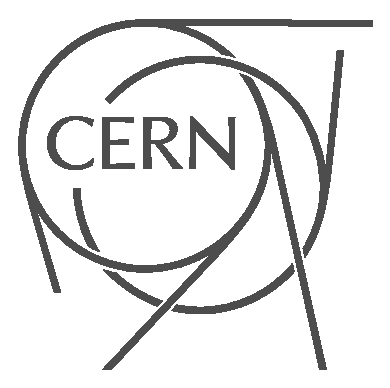
\includegraphics[height=1.2cm]{cern-logo-gray.eps}}
\sbox{\pilogo}{\includegraphics[height=0.75cm]{cern-logo.eps}}
\sbox{\lhcblogo}{
\includegraphics[height=0.75cm]{lhcb-logo.eps}}

\setbeamertemplate{footline}
{
  \leavevmode%
  \hbox{%
  \begin{beamercolorbox}[wd=.333333\paperwidth,ht=2.25ex,dp=1ex,left]{author in head/foot}%
    \usebeamerfont{author in head/foot}\vtop{\vskip-2.25ex\hbox{\resizebox{!}{3.25ex}{\usebox{\pilogo}}}}%
    \hfill \insertshortauthor~~(\insertshortinstitute) \hfill%
  \end{beamercolorbox}%
  \begin{beamercolorbox}[wd=.333333\paperwidth,ht=2.25ex,dp=1ex,center]{title in head/foot}%
    \usebeamerfont{title in head/foot}\insertshorttitle%
  \end{beamercolorbox}%
  \begin{beamercolorbox}[wd=.333333\paperwidth,ht=2.25ex,dp=1ex,right]{date in head/foot}%
    \usebeamerfont{date in head/foot}\insertshortdate{}\hspace*{2em}%
    \insertframenumber{} / \inserttotalframenumber\hspace*{2ex} \vtop{\vskip-2.25ex\hbox{\resizebox{!}{3.25ex}{\usebox{\lhcblogo}}}}%
  \end{beamercolorbox}}%
  \vskip0pt%
}

\setbeamertemplate{frametitle}
{
  \ifbeamercolorempty[bg]{frametitle}{}{\nointerlineskip}%
  \leavevmode%
  \vskip-2pt\hbox{%
  \begin{beamercolorbox}[wd=\paperwidth,left]{frametitle}%
    \usebeamerfont{frametitle}%
    \vskip.125ex%
    \hbox{\vtop{\raisebox{-1ex}[1ex][1ex]{\makebox[0pt][l]{\usebox{\unilogo}}}%
    \hspace{1em}\strut\insertframetitle\strut}\par%
    {%
      \ifx\insertframesubtitle\@empty%
      \else%
      {\usebeamerfont{framesubtitle}\usebeamercolor[fg]{framesubtitle}\insertframesubtitle\strut\par}%
      \fi
    }}%
  \end{beamercolorbox}%
  }%
}


\definecolor{bandgreen}{rgb}{0.4,0.8,0.4}
\newcommand{\FIXME}{{\color{red}FIXME}}
\newcommand{\arxiv}[1]{{\color{gray}\tiny$[$\href{http://arxiv.org/abs/#1}{arXiv:#1}$]$}}
\newcommand{\jref}[2]{{\color{gray}\tiny$[$\href{#2}{#1}$]$}}

\author[M. Schiller]{Manuel Schiller}
\institute{CERN}
\date{July 9th-10th, 2015}
\title{Getting started with B2DXFitters}

\begin{document}
\begin{fmffile}{talk-fmf}
\section[1st B2DXFitters workshop]{$\,$}
\subsection{Padova}
\maketitle

\section{setting things up}
\begin{frame}{}
    \vfill
    
\includegraphics[width=.995\textwidth]{modelgraph} \\
    $\,$ \hfill PDF structure of the $1\textsf{ fb}^{-1}$ $B^0_s\rightarrow
    D_s^\mp K^\pm$ cFit\hfill $\,$ \\
    \vfill
\end{frame}

\begin{frame}{setting things up}
\begin{itemize}
\item before we can get started, we have to set up the environment
\begin{itemize}
\item {\tt B2DXFitters} is light in its requirements:
\begin{itemize}
\item ROOT (recent 5.34 or 6.02 release or newer) and gmake are enough\\
    ({\color{blue} standalone builds on your laptop!})
\item you can (of course) also use an LHCb environment \\
    (Urania/Erasmus/DaVinvi/\ldots)
\end{itemize}
\item will briefly go into both\ldots 
\end{itemize}
\item for writing your own code, have to load the right libraries
\end{itemize}
\end{frame}

\subsection{setup in LHCb environment}
\begin{frame}{setup in LHCb environment}
    \vfill
    $\,$ \hfill {\Huge setup in LHCb environment} \hfill $\,$ \\
    \vfill
\end{frame}

\begin{frame}[fragile]{setup in LHCb environment (1/2)} \small
this follows the usual pattern when you compile LHCb software:
\begin{itemize}
\item set up environment for building
\begin{lstlisting}[language=sh]
> SetupProject --build-env Urania v3r0
Build-time environment for Urania v3r0 ready.
Created user project in /home/mala/cmtuser/Urania_v3r0
Current directory is '/home/mala/cmtuser/Urania_v3r0'.
Using CMTPROJECTPATH = '/home/mala/cmtuser:/local/lhcb:/local/lcg/releases:/local/lcg/app/releases:/local/lcg/external'
\end{lstlisting}
\item getpack UraniaSys and B2DXFitters
\begin{lstlisting}[language=sh]
> getpack UraniaSys v3r0
....
A    UraniaSys/CMakeLists.txt
Checked out revision 191429.
Checked out package UraniaSys v3r0 (1/1)
Processed packages:
        UraniaSys       v3r0
> getpack PhysFit/B2DXFitters head
....
A    PhysFit/B2DXFitters/CMakeLists.txt
Checked out revision 191429.
Checked out package PhysFit/B2DXFitters head (1/1)
Processed packages:
        PhysFit/B2DXFitters     head
\end{lstlisting}
\end{itemize}
\end{frame}

\begin{frame}[fragile]{setup in LHCb environment (2/2)} \small
this follows the usual pattern when you compile LHCb software:
\begin{itemize}
\item add B2DXFitters to cmt/requirements of Urania
\begin{lstlisting}[language=sh]
> echo "use B2DXFitters v* PhysFit" >> UraniaSys/cmt/requirements
\end{lstlisting}
\item configure packages
\begin{lstlisting}[language=sh]
> for i in UraniaSys PhysFit/B2DXFitters; do (cd $i/cmt; cmt config); done
\end{lstlisting}
\item source setup.sh to set up environment
\begin{lstlisting}[language=sh]
> source ./UraniaSys/cmt/setup.sh
\end{lstlisting}
\item compile everything
\begin{lstlisting}[language=sh]
> cd $URANIASYSROOT/cmt; cmt br make -j8
\end{lstlisting}
\item start hacking\footnote{diversity is important, so emacs or similar tools
    are permissible ;)}\ldots
\begin{lstlisting}[language=sh]
> cd $B2DXFITTERSROOT
> source $URANIASYSROOT/cmt/setup.sh
> vim ...
\end{lstlisting}
\end{itemize}
\end{frame}

\subsection{standalone setup}
\begin{frame}{standalone setup}
    \vfill
    $\,$ \hfill {\Huge standalone setup} \hfill $\,$ \\
    \vfill
\end{frame}

\begin{frame}[fragile]{standalone setup} \small
\begin{itemize}
\item useful when you don't want/need all that LHCb software crap
\item requirements
\begin{itemize}
\item *nix system with recent C++ compiler (C++11)
\item recent ROOT (6.02 or newer, or a recent 5.34 version) with RooFit and
    Minuit compiled in
\item for ROOT 5.34:
\begin{itemize}
\item gccxml, ROOT compiled with reflex support
\end{itemize}
\item GNU Make
\end{itemize}
\item make sure you can start ROOT from your command line
\item check out and compile:
\begin{lstlisting}[language=sh]
> svn co svn+ssh://svn.cern.ch/reps/lhcb/Urania/trunk/PhysFit/B2DXFitters B2DXFitters
...
> cd B2DXFitters/standalone
> make -j4
...
> source setup.sh
\end{lstlisting}
\item start hacking\ldots
\end{itemize}
\end{frame}

\section{loading libraries}
\begin{frame}{loading libraries}
    \vfill
    $\,$ \hfill {\Huge loading libraries} \hfill $\,$ \\
    \vfill
\end{frame}

\subsection{C++}
\begin{frame}[fragile]{C++}
\begin{itemize}
\item if you write your own C++ macros, this is what you have to do:
\begin{itemize}
\item only ROOT 5:
\begin{lstlisting}[language=C++]
#include "Cintex/Cintex.h"
gSystem->Load("libReflex");
gSystem->Load("libCintex");
ROOT::Cintex::Cintex::Enable();
\end{lstlisting}
\item then in all ROOT versions:
\begin{lstlisting}[language=C++]
gSystem->Load("libRooFit");
\end{lstlisting}
\item then, depending on
\begin{itemize}
\item standalone environment
\begin{lstlisting}[language=C++]
gSystem->Load("/full/path/to/B2DXFitters/standalone/libB2DXFitters");
\end{lstlisting}
\item LHCb software environment
\begin{lstlisting}[language=C++]
gSystem->Load("/full/path/to/B2DXFitters/x86_64-slc6-gcc48-opt/libB2DXFittersDict");
gSystem->Load("/full/path/to/B2DXFitters/x86_64-slc6-gcc48-opt/libB2DXFittersLib");
\end{lstlisting}
\end{itemize}
\end{itemize}
\end{itemize}
\end{frame}

\subsection{Python}
\begin{frame}[fragile]{Python}
\begin{itemize}
\item for standalone scripts ({\tt chmod 755}) copy the prolog in {\tt
	scripts/prolog.py} to the start of your script
\begin{itemize}
\item handles all the ROOT 5/6, LHCb/stanalone environment issues
\item will find and load the correct libraries
\item set up a few useful tweaks (jemalloc/tcmalloc, ulimits)
\end{itemize}
\item in all python code, include this at the start:
\begin{lstlisting}[language=Python]
import B2DXFitters                                                                                                                                                                              
import ROOT                                                                                                                                                                                     
from ROOT import RooFit 
\end{lstlisting}
\item much easier than the C++ version, right? \\
    I guess you wanted to code in python all along\ldots
\end{itemize}
\end{frame}

\section{package structure}
\begin{frame}{package structure}
    \vfill
    $\,$ \hfill {\Huge package structure} \hfill $\,$ \\
    \vfill
\end{frame}

\begin{frame}{reminder: package structure}
\begin{itemize}
\item important to understand package structure (subdirectories):
\begin{center}\small \begin{tabular}{l l}
B2DXFitters & header files for C++ algorithms \\
    cmt & used for cmt (building) \\
    data & various data files (templates), config files \\
    dict & ROOT dictionaries (reflection information) \\
    doc & release.notes, other documentation \\
    python & reusable python code \\
    scripts & fitting (python) scripts \\
    src & C++ sources \\
    standalone & standalone build dir (symlinks to src/*.cxx) \\
    tutorial & material for hands-on session (feel free to add!) \\
\end{tabular} \end{center}
\item looking for RooFit classes: {\color{blue} B2DXFitters, src (, standalone)}
\item looking for reusable parts of fit: {\color{blue} python/B2DXFitters}
\item concrete fit implementations: {\color{blue} scripts}
\end{itemize}
\end{frame}

\section{hands-on session time fit}
\begin{frame}{hands-on session time fit}
    \vfill
    $\,$ \hfill {\Huge hands-on session time fit} \hfill $\,$ \\
    \vfill
\end{frame}

\begin{frame}{hands-on session time fit}
\begin{itemize}
\item now you know how to set things up, and where things are
\item now we can start the tour\ldots
\end{itemize}
\end{frame}

\begin{frame}{time fit hands-on session}
\begin{itemize}
\item five examples in {\tt tutorial}\footnote{please {\tt svn up}}:
\begin{itemize}
\item {\tt time-tut000.py}: average $\eta$, perfect $\sigma_t$, no acceptance
\item {\tt time-tut001.py}: average $\eta$, $\sigma_t$, no acceptance
\item {\tt time-tut002.py}: average $\eta$, $\sigma_t$, spline acceptance
\item {\tt time-tut003.py}: per-event $\eta$, average $\sigma_t$, spline acceptance
\item {\tt time-tut004.py}: per-event $\eta$, $\sigma_t$, spline acceptance
\end{itemize}
\end{itemize}
\end{frame}

\begin{frame}{{\tt time-tut000.py}}
\begin{itemize}
\item {\tt time-tut000.py}: average $\eta$, perfect $\sigma_t$, no acceptance
\item suggestions
\begin{itemize}
\item look at it
\item notice the config file reading functions from {\tt B2DXFitters.utils}
\item generation and fit pdfs separate
\item pdf and fit result written to ROOT files
\item run it: {\tt ./time-tut000.py SEED}
\end{itemize}
\item next steps:
\begin{itemize}
\item add average $\sigma_t$ (use yesterday's slides as a guide)
\end{itemize}
\end{itemize}
\end{frame}

\begin{frame}{{\tt time-tut001.py}}
\begin{itemize}
\item {\tt time-tut001.py}: average $\eta$, $\sigma_t$, no acceptance
\item suggestions
\begin{itemize}
\item look at it
\item have a good look at {\tt setConstantIfSoConfigured}
\item let's play with/discuss settings for Optimize, NumCPU\ldots
\item maybe can discuss settings for numerical integration (on the side\ldots)
\item run it: {\tt ./time-tut001.py SEED}
\end{itemize}
\item next steps:
\begin{itemize}
\item add spline acceptance (use yesterday's slides as a guide)
\end{itemize}
\end{itemize}
\end{frame}

\begin{frame}{{\tt time-tut002.py}}
\begin{itemize}
\item {\tt time-tut002.py}: average $\eta$, $\sigma_t$, spline acceptance
\item suggestions
\begin{itemize}
\item look at it
\item biggest change: PDF builder function for separate PDFs for generation
    and fitting
\item look into ROOT files saved
\item let's discuss the blinding mechanism
\item familiarise yourself with {\tt scripts/printFitResult.py}
\item run it: {\tt ./time-tut002.py SEED}
\end{itemize}
\item next steps:
\begin{itemize}
\item add per-event $\eta$ (use yesterday's slides as guide)
\end{itemize}
\end{itemize}
\end{frame}

\begin{frame}{hint on mistag distributions}
\begin{itemize}
\item for toys, often you want something quick and dirty, no need for full template
\begin{center}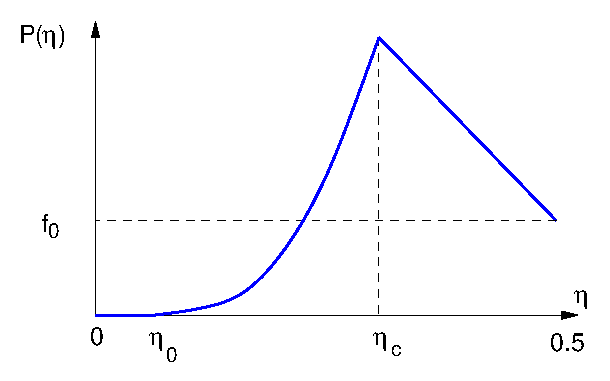
\includegraphics[width=.49\textwidth]{trivialmistag}\end{center}
\item {\tt MistagDistribution} has roughly right shape
\item can tune average mistag of distribution as parameter:
\begin{itemize}
\item zero up to $\eta_0$ -- try $\eta_0=0.07$
\item then quadratic until $\eta_c$
\item then linear to point $(0.5, f)$ -- try $f=0.25$
\item tunes $\eta_c$ to get desired average, e.g. 0.35
\end{itemize}
\end{itemize}
\end{frame}

\begin{frame}{{\tt time-tut003.py}}
\begin{itemize}
\item {\tt time-tut003.py}: per-event $\eta$, average $\sigma_t$, spline acceptance
\item suggestions
\begin{itemize}
\item look at it
\item familiarise yourself with {\tt scripts/make\_histos.py} (pull and
    residual plots)
\item run it: {\tt ./time-tut003.py SEED}
\end{itemize}
\item next steps:
\begin{itemize}
\item add per-event $\sigma_t$ (use yesterday's slides as a guide)
\end{itemize}
\end{itemize}
\end{frame}

\begin{frame}{hint on mistag distributions}
\begin{itemize}
\item again, for simple toys, you may not need a template
\item can use
    \[ P(\sigma_t)\sim\sigma_t^6\,e^{-\frac{\sigma_t}{\sigma_{avg} / 7}} \]
\begin{center}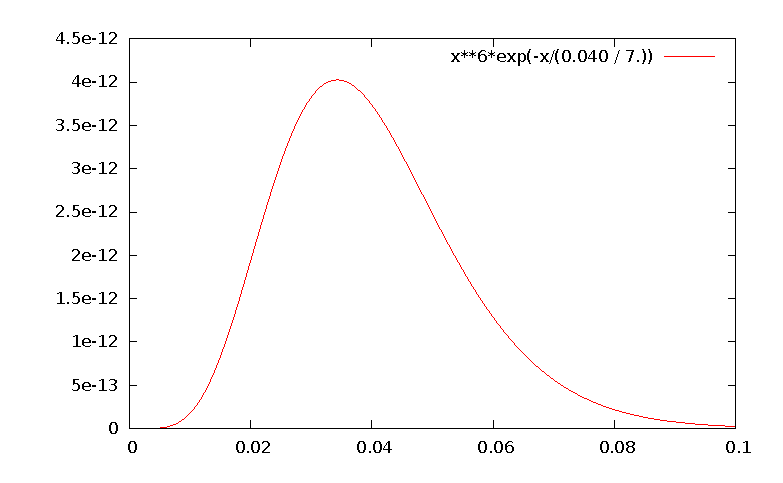
\includegraphics[width=.49\textwidth]{sigmat}\end{center}
\item has about the right shape, can tune expectation value ($\sigma_{avg}$)
\end{itemize}
\end{frame}

\begin{frame}{{\tt time-tut004.py}}
\begin{itemize}
\item {\tt time-tut004.py}: per-event $\eta$, $\sigma_t$, spline acceptance
\item suggestions
\begin{itemize}
\item look at it
\item run it: {\tt ./time-tut004.py SEED}
\end{itemize}
\item next steps:
\begin{itemize}
\item now you are ready to look at the ``big beasts of the plain'', \\
    {\tt scripts/runBs2DsKCPAsymmObsFitter-cFit.py} ($D_sK$ cFit) and \\
    {\tt scripts/plotBs2DsHTimeModels.py }
\begin{itemize}
\item these are much uglier than the the examples (real world, you know\ldots
    ;)
\item if you've worked through the examples, you have all the tools you need
    to build your own fit (and look at the cFit to see what not to do)
\end{itemize}
\end{itemize}
\end{itemize}
\end{frame}

\begin{frame}{conclusion}
\begin{itemize}
\item that's it
\begin{itemize}
\item let me know what was useful (or not useful)
\item open to all kinds of suggestions (more/different material, presentation
    style, wishlist\ldots)
\end{itemize}
\end{itemize}
\end{frame}

\end{fmffile}

\end{document}

% vim: sw=4:tw=78:ft=tex
